\documentclass{../../fal_assignment}
\graphicspath{ {../../} }

\usepackage{enumitem}
\setlist{nosep} % Make enumerate / itemize lists more closely spaced
\usepackage[T1]{fontenc} % http://tex.stackexchange.com/a/17858
\usepackage{url}
\usepackage{todonotes}

\title{Creative Computing Tasks [REFER]}
\author{Dr Umaima Haider and Joseph Walton-Rivers}
\module{COMP280}
\version{1.0}

\begin{document}

\maketitle

\section*{Introduction}

\begin{marginquote}
``No matter the language, learning to program will take a very long time, and is often very frustrating. I'm sorry. There is no solution. Just practice. Regular practice.

``That's why I always call programming a craft. You spend your life honing your craft, not a weekend.

``You WILL get stuck.
You WILL get very frustrated.
You WILL want to quit.
You WILL think this is all pointless and dumb.
You WILL look at the things others are doing and think `How the hell am I going to do this?'

``Programming can make you feel empowered.
Programming can make you feel excited.
Programming can be a major source of inspiration.

``But it has to come from you. YOU are the driving force here. I and others can only point you in a direction.''

\par --- \'Olafur Waage
\end{marginquote}
\marginpicture{flavour_pic}{
    \emph{SpaceChem} is a puzzle game in which players must apply computational thinking to build circuits which assemble
    chemical molecules.
}

In this assignment, you are required to complete a number of tasks to construct a portfolio demonstrating your mastery of different specialisms within the area of creative computing. These being: networking; artificial intelligence; optisation; and human-computer interaction. To help you structure your portfolio, the assignment is divided into a series of bite-sized \textbf{worksheets}. The worksheets require you to \textbf{recognise}, \textbf{analyse}, \textbf{design}, \textbf{annotate}, and \textbf{write} a series of computer programs according to instructions, as well as to \textbf{solve} problems.

In order for programmers to communicate with each other regarding the technical aspects of a game development project, they must have good computational thinking skills, a strong foundational knowledge of computing principles, applied knowledge of program design notations and annotations, and a working knowledge of particular programming constructs (often as a result of writing their own versions). Such knowledge and skills take time and a sustained effort to develop. For this resubmission, you will re-recreate the work you submitted originally.

This assignment is formed of \textbf{FOUR} parts: Worksheets 1 to 4. These address the following tasks:

\begin{enumerate}
  \item \textbf{Recognise} basic networking concepts and \textbf{analyse} some of these concepts in the cloud environment;
  \item \textbf{Implement} a decision-making artifical intelligence technique (e.g. behaviour trees)
  \item \textbf{Select} a previouslly written application or algorithm, and then follow an \textbf{optimisation} process to ensure the code is running as \textbf{efficently} as possible
  \item and \textbf{conduct} a heuristic analysis of a game in order to \textbf{evaluate} its usability.
\end{enumerate}

For each part you must:

\begin{enumerate}[label=(\roman*)]
    \item \textbf{Read} the instructions in the worksheet;
    \item \textbf{Complete} all of the problems presented;
    \item \textbf{Submit} your solution according to the instructions on the worksheet, and by the deadline specified on the worksheet.
\end{enumerate}

\subsection*{Assignment Setup} 

This assignment consists of a \textbf{single summative submission}.

Each worksheet contains detailed submission instructions for their components. By the deadline you will be required make a final summative submission of all four of your worksheet solutions.

Prepare a \textbf{single \texttt{.zip} file} containing your submissions \textbf{in separate folders}, and upload it to the appropriate submission area on LearningSpace. The folder structure within your \texttt{zip} file should resemble that shown in Figure~\ref{fig:folder_structure}.

\begin{figure}
    \begin{center}
        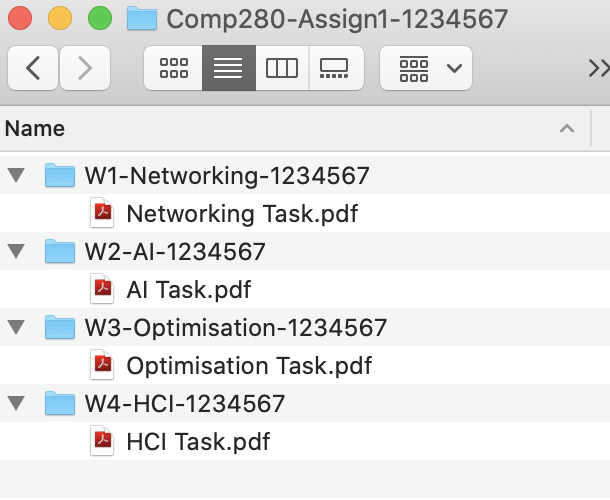
\includegraphics[height=0.4\textheight]{folder_structure}
    \end{center}
    \caption{Recommended folder structure for your final summative submission.}
    \label{fig:folder_structure}
\end{figure}

\textbf{This final submission is subject to the usual university policies regarding late submission or non-submission,
as detailed in the course handbook --- failure to make a submission via LearningSpace by the summative deadline will
 be subject to penalties.}

\section*{Additional Guidance}

Make a submission on time and you will get a basic pass on that worksheet,
even if your solution is incorrect or incomplete.
A solution meeting all of the correctness and/or functionality criteria on the worksheet is required to demonstrate basic proficiency,
with higher grades contingent on your solution being of a high quality.
The individual worksheets give more guidance as to what constitutes ``quality'' for that particular exercise,
but bear in mind that a major purpose of these worksheets is to assess your ability to communicate
complex computational ideas in English, in notation and in program code.
Thus pay particular attention to the precision and clarity of your written communication,
and the readability and maintainability of your source code.

The underlying skills being developed are also critically important to your progression as a programmer, so do not neglect the work.
Do not underestimate the time it takes to complete tasks that may appear trivial when you first see them.
Do not leave work until the last minute! With programming in particular, trying to ``cram'' the work just before the deadline is a sure path to failure.

A key skill of software development is the ability to read and follow instructions.
Make sure to read the worksheet carefully to ensure that you are meeting all of the requirements ---
a surprising number of students needlessly lose marks by misreading the worksheet.

Nobody learns in a vacuum: you are allowed, and indeed encouraged, to discuss your work with your peers. However you must be very careful to avoid falling into \textbf{academic misconduct}, in particular \textbf{plagiarism}. If any part of your solution is \textbf{not your own individual work}, you must make this as clear as possible in your submission, for example in source code comments.

\section*{FAQ}

\begin{itemize}
	\item 	\textbf{What is the deadline for this assignment?} \\ 
			Falmouth University policy states that summative deadlines must only be specified on the MyFalmouth system.
    		
	\item 	\textbf{What should I do to seek help?} \\ 
    		You can email your tutor for informal clarifications.
    		
	\item 	\textbf{How will I receive feedback on my work?} \\ 
    		You will be given written feedback after submission.
    		If you require more in-depth feedback or discussion, please book an appointment with your tutor.
\end{itemize}


\section*{Worksheet Rubrics and Weightings}
Each worksheet is marked according to its own rubric. Please see individual worksheets for details.

Each of the four worksheets is \textbf{weighted equally}, and so is worth 33.3\% as the overall mark will consist of the combined (overall) mark will consist of the marks for the three highest scoring worksheets.

The worksheets are the same as the first attempt worksheets. Please note as this is a referral brief, there will not be formative deadlines for the worksheets and mentions of these in the worksheets should be deregarded.

\end{document}
